\documentclass{beamer}
% %- http://www.graphpad.com/guides/prism/6/curve-fitting/index.htm?reg_spline_and_lowess_curves.htm
\usepackage{subfiles}
\usepackage{framed}
\begin{document}
	%=========================================================%
\section{LOWESS LOESS}
\begin{frame}
	\frametitle{LOWESS LOESS}
	\large
	\begin{itemize}
		\item \textbf{LOESS} and \textbf{LOWESS} (locally weighted scatterplot smoothing) are two strongly related non-parametric regression methods that combine multiple regression models in a k-nearest-neighbor-based meta-model.
		\item  "LOESS" is a later generalization of LOWESS; although it is not a true initialism, it may be understood as standing for "\textit{\textbf{LOcal regrESSion}}".
		
	\end{itemize}
\end{frame}
%========================================================= %
\begin{frame}\frametitle{LOWESS LOESS}\large	
	\begin{itemize}
		\item LOESS and LOWESS thus build on "classical" methods, such as linear and nonlinear least squares regression. They address situations in which the classical procedures do not perform well or cannot be effectively applied without undue labor.
		\item LOESS combines much of the simplicity of linear least squares regression with the flexibility of nonlinear regression. 
		\item It does this by fitting simple models to localized subsets of the data to build up a function that describes the deterministic part of the variation in the data, point by point. 
		\item In fact, one of the chief attractions of this method is that the data analyst is not required to specify a global function of any form to fit a model to the data, only to fit segments of the data.
	\end{itemize}
\end{frame}

\begin{frame}
\frametitle{Loess}
	\begin{figure}
\centering
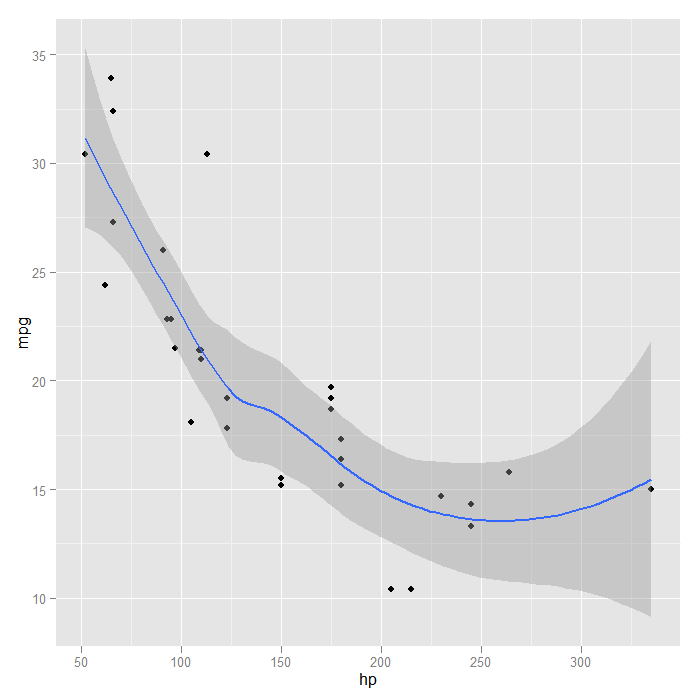
\includegraphics[width=0.8\linewidth]{images/ggplot2loess}

\end{figure}

\end{frame}
%========================================== %
\begin{frame}
	\begin{figure}
\centering
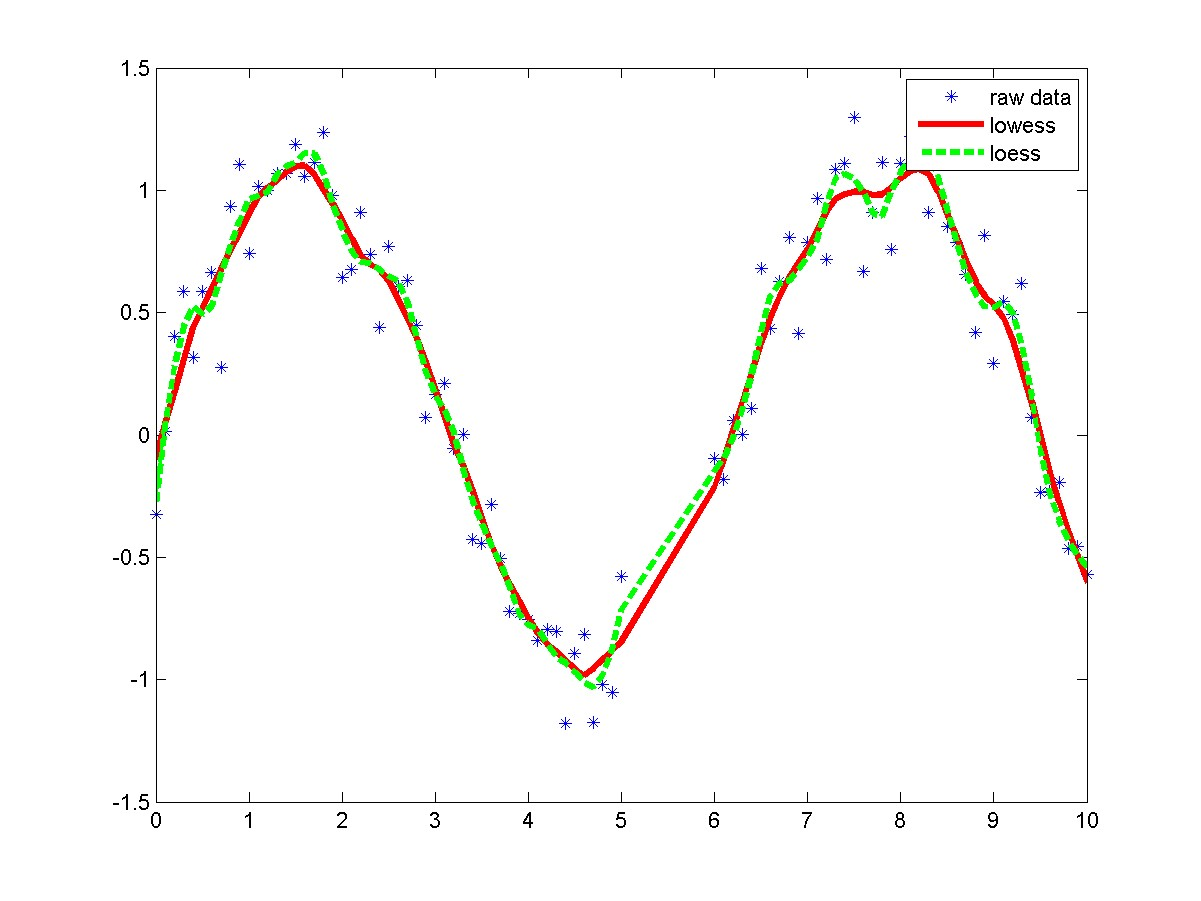
\includegraphics[width=1\linewidth]{images/loesslowess}
\caption{}
\label{fig:loesslowess}
\end{figure}

\end{frame}
%====================================================== %


\section{Ridge Regression}
\begin{frame}
\large
\frametitle{5. Ridge Regression}
	\begin{itemize}
	\item Ridge Regression is a technique used when the data suffers from \textbf{multicollinearity} ( independent variables are highly correlated).
	\item  In multicollinearity, even though the least squares estimates (OLS) are unbiased, their variances are large which deviates the observed value far from the true value.
	\item By adding a degree of bias to the regression estimates, ridge regression reduces the standard errors.
	\end{itemize}

\end{frame}
%==============================================================================%
\begin{frame}[fragile]
	
	Above, we saw the equation for linear regression. Remember? It can be represented as:
	
\[	y=a+ b*x\]
	
	This equation also has an error term. The complete equation becomes:
	
	\begin{verbatim}
	y=a+b*x+e (error term),  [error term is the value needed to correct for a prediction error between the observed and predicted value]
	=> y=a+y= a+ b1x1+ b2x2+....+e, for multiple independent variables.
	\end{verbatim}

\end{frame}
%==============================================================================%
\begin{frame}
	\begin{itemize}
		\item In a linear equation, prediction errors can be decomposed into two sub components. 
		\item First is due to the biased and second is due to the variance. 
		\item Prediction error can occur due to any one of these two or both components. Here, we’ll discuss about the error caused due to variance.
	\end{itemize}
\end{frame}
%==============================================================================%
\begin{frame}
	\frametitle{Ridge Regression}
	\large
	Ridge regression solves the multicollinearity problem through shrinkage parameter $\lambda$ (lambda). Look at the equation below.
	
	Ridge
	
	In this equation, we have two components. First one is least square term and other one is lambda of the summation of β2 (beta- square) where β is the coefficient. This is added to least square term in order to shrink the parameter to have a very low variance.
\end{frame}
%==============================================================================%
\begin{frame}
	\frametitle{Ridge Regression}
	\large	
	Important Points:
	
	\begin{itemize}
\item 	The assumptions of this regression is same as least squared regression except normality is not to be assumed
\item 	It shrinks the value of coefficients but doesn’t reaches zero, which suggests no feature selection feature
\item  	This is a regularization method and uses l2 regularization.
	\end{itemize}

	
\end{frame}
\section{Regularization}
%- http://stats.stackexchange.com/questions/4961/what-is-regularization-in-plain-english

%================================================== %
\begin{frame}
	\frametitle{Regularization}
	\large
	\begin{itemize}
\item In simple terms, regularization is tuning or selecting the preferred level of model complexity so your models are better at predicting (generalizing). 
\item If you don't do this your models may be too complex and overfit or too simple and underfit, either way giving poor predictions.
	\end{itemize}

\end{frame}
%================================================== %
\begin{frame}
	\frametitle{Regularization}
	\large
	\begin{itemize}
\item If you least-squares fit a complex model to a small set of training data you will probably overfit, this is the most common situation. 
\item The optimal complexity of the model depends on the sort of process you are modeling and the quality of the data, so there is no a-priori correct complexity of a model.
	\end{itemize}

\end{frame}
%================================================== %
\begin{frame}
	\frametitle{Regularization}
	\large
To regularize you need 2 things:

\begin{itemize}
\item A way of testing how good your models are at prediction, for example using cross-validation or a set of validation data (you can't use the fitting error for this).
\item A tuning parameter which lets you change the complexity or smoothness of the model, or a selection of models of differing complexity/smoothness.
\end{itemize}

\end{frame}
%================================================== %
\begin{frame}
	\frametitle{Regularization}
	\large
Basically you adjust the complexity parameter (or change the model) and find the value which gives the best model predictions.
Note that the optimized regularization error will not be an accurate estimate of the overall prediction error so after regularization you will finally have to use an additional validation dataset or perform some additional statistical analysis to get an unbiased prediction error.

An alternative to using (cross-)validation testing is to use Bayesian Priors or other methods to penalize complexity or non-smoothness, but these require more statistical sophistication and knowledge of the problem and model features.
\end{frame}
\section{Lasso Regression}
%==============================================================================%
\begin{frame}
	\frametitle{6. Lasso Regression}
	\begin{itemize}
\item Similar to Ridge Regression, Lasso (Least Absolute Shrinkage and Selection Operator) also penalizes the absolute size of the regression coefficients. 
\item In addition, it is capable of reducing the variability and improving the accuracy of linear regression models.  
\item Look at the equation below: LassoLasso regression differs from ridge regression in a way that it uses absolute values in the penalty function, instead of squares.
	\end{itemize}
	 
	
\end{frame}
%============================================================ %
\begin{frame}
	\frametitle{Lasso Regression}
	In statistics and statistical and machine learning, lasso (least absolute shrinkage and selection operator) (also Lasso or LASSO) is a regression analysis method that performs both variable selection and regularization in order to enhance the prediction accuracy and interpretability of the statistical model it produces. It was introduced by Robert Tibshirani in 1996 based on Leo Breiman’s Nonnegative Garrote.[1][2] 
	
\end{frame}
%============================================================ %
\begin{frame}
	\frametitle{Lasso Regression}
	lasso was originally formulated for least squares models and this simple case reveals a substantial amount about the behavior of the estimator, including its relationship to ridge regression and best subset selection and the connections between lasso coefficient estimates and so-called soft thresholding. It also reveals that (like standard linear regression) the coefficient estimates need not be unique if covariates are collinear.
\end{frame}
\begin{frame}
	\begin{figure}
\centering
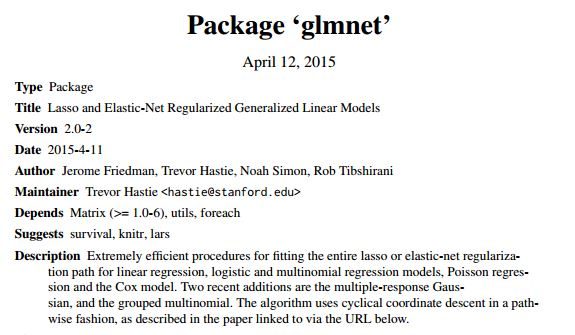
\includegraphics[width=0.9\linewidth]{images/CRAN-glmnet}
\end{figure}

\end{frame}
%==============================================================================%
\begin{frame}
	\frametitle{6. Lasso Regression}
	\large
	\begin{itemize}
\item 	This leads to penalizing (or equivalently constraining the sum of the absolute values of the estimates) values which causes some of the parameter estimates to turn out exactly zero. 
\item Larger the penalty applied, further the estimates get shrunk towards absolute zero. 
\item This results to variable selection out of given n variables.
	\end{itemize}

\end{frame}
%==============================================================================%
\begin{frame}
	\frametitle{6. Lasso Regression}
	\large
	Important Points:
	\begin{itemize}
\item 	The assumptions of this regression is same as least squared regression except normality is not to be assumed
\item 	It shrinks coefficients to zero (exactly zero), which certainly helps in feature selection
\item 	This is a regularization method and uses l1 regularization
\item 	If group of predictors are highly correlated, lasso picks only one of them and shrinks the others to zero
	\end{itemize}

\end{frame}
%=======================================================%

\section{Elastic Net}
\begin{frame}
	\frametitle{Elastic Net}
	\begin{itemize}
	\item ElasticNet is hybrid of Lasso and Ridge Regression techniques. 
	\item It is trained with L1 and L2 prior as regularizer. Elastic-net is useful when there are multiple features which are correlated. 
	\item Lasso is likely to pick one of these at random, while elastic-net is likely to pick both.
	\end{itemize}
	
\end{frame}
%========================================================= %
\begin{frame}
	\frametitle{7. ElasticNet Regression}

	
%	Elastic_Net
	\begin{itemize}
\item 	A practical advantage of trading-off between Lasso and Ridge is that, it allows Elastic-Net to inherit some of Ridge’s stability under rotation.
	\end{itemize}

\end{frame}
%==============================================================================%
\begin{frame}
	\frametitle{7. ElasticNet Regression}
	Important Points:
	
	It encourages group effect in case of highly correlated variables
	There are no limitations on the number of selected variables
	It can suffer with double shrinkage
	Beyond these 7 most commonly used regression techniques, you can also look at other models like Bayesian, Ecological and Robust regression.
	%==============================================================================%
	
\end{frame}

\begin{frame}
	\begin{figure}
\centering
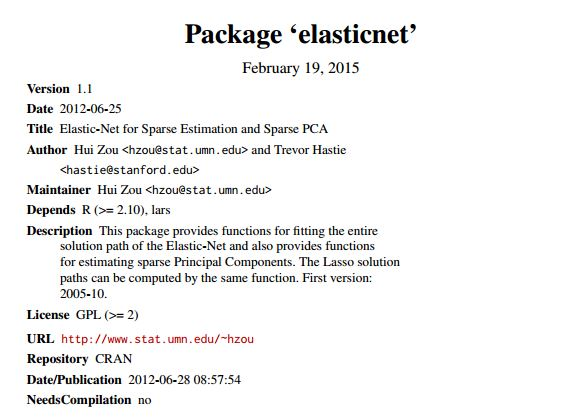
\includegraphics[width=1.05\linewidth]{images/CRAN-elasticnet}

\end{figure}

\end{frame}
%========================================================== %
\begin{frame}
\frametitle{Boston Data Set}
\begin{figure}
\centering
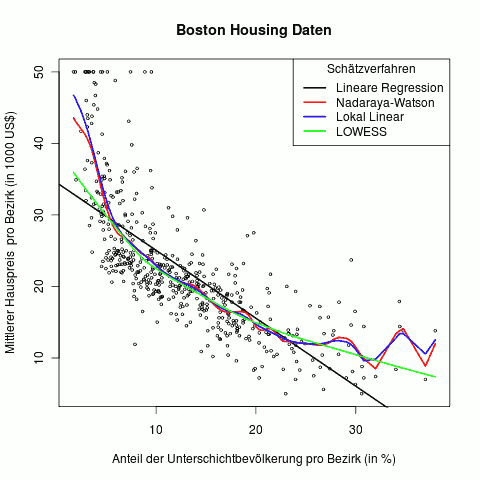
\includegraphics[width=0.8\linewidth]{images/LocalPolynomialRegression}


\end{figure}
\end{frame}
%===================================================== %
\section{Quantile Regression}
% %-https://en.wikibooks.org/wiki/R_Programming/Quantile_Regression
\begin{frame}
	\begin{itemize}
\item 	Quantile regression is a type of regression analysis used in statistics and econometrics. Whereas the method of least squares results in estimates that approximate the conditional mean of the response variable given certain values of the predictor variables, quantile regression aims at estimating either the conditional median or other quantiles of the response variable.
	
\item 	R offers several packages that implement quantile regression, most notably quantreg by Roger Koenker,but also gbm,and quantregForest.
	\end{itemize}

\end{frame}
%======================================================== %

\begin{frame}
\frametitle{Quantile Regression}
\large
	\begin{figure}
\centering
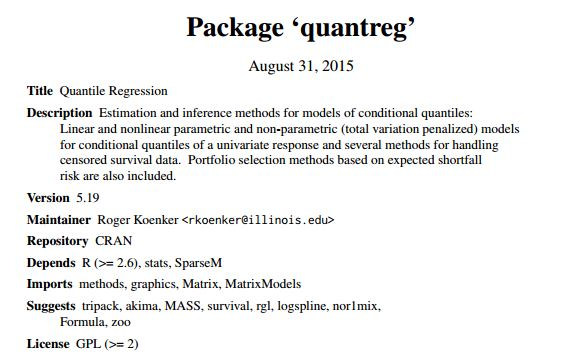
\includegraphics[width=0.7\linewidth]{images/CRAN-quantreg}

\end{figure}

\end{frame}
%========================================================== %

\begin{frame}
	\frametitle{Quantile Regression}
	\large
	\begin{figure}
\centering
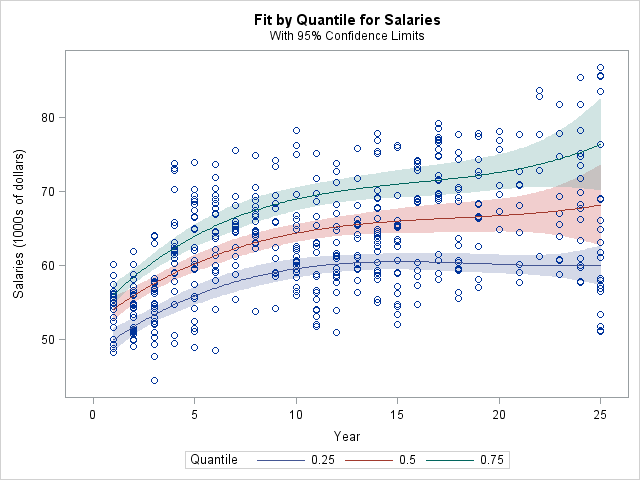
\includegraphics[width=0.7\linewidth]{images/quantregbin3}
\caption{}
\label{fig:quantregbin3}
\end{figure}

\end{frame}
%======================================================= %
\section{Kernel Regression}
\begin{frame}
\frametitle{Kernel Regression}
\large\noindent \textbf{Nadaraya-Watson Kernel Regression}\\
	Nadaraya 1964 and Watson 1964 proposed to estimate m as a locally weighted average, using a kernel as a weighting function.\\ The Nadaraya-Watson estimator is:
	
	\[\widehat{m}_h(x)=\frac{\sum_{i=1}^n K_h(x-x_i) y_i}{\sum_{i=1}^nK_h(x-x_i)}  \]
	
	where K is a kernel with a bandwidth h. The fraction is a weighting term with sum 1.
\end{frame}

%========================================================= %

\end{document}
